% !TEX root = /Users/zhuzhuangdi/Desktop/MSUCourses/MachineLearning847/17spr_wang_zhu_du/Final/final_report.tex
\section{Evalutaion}
For each of the three approaches, we use the same preprocessing steps to get the same features. Then we compare among the  Song Ci generated from the three approaches based on three metrics : structure, rhyme, and semantics. 

% !TEX root = /Users/zhuzhuangdi/Desktop/MSUCourses/MachineLearning847/17Project/17spr_wang_zhu_du/Middle/middle_report.tex
\section{Data Description}   
For our experiment, we obtained dataset for both Tang Shi and Song Ci. Many research were conducted for automatically generating Tang Shi. So we can evaluate our experiment result by comparing with these machine-created Tang Shi. And then we can move forward to Song Ci.
\subsubsection{Tang Poetry Corpus}
We use Quan Tangshi as our Tang Poetry corpus.\cite{1960quantangshi}. It was commissioned by Yin Cao in 1705 and published under the name of Kangxi Emperor. It contains 49,000 lyric poems (in the dataset we used it has 49,274 poems) and is believed the largest collection of Tang poetry. We obtained the dataset from the server of \cite{zhang2014chinese}.
\subsubsection{Song Ci Corpus} 

\subsection{Implementation of Genetic Algorithm}
Initially, we collect additional information about syntactic pattern of sentences with different length, format of tone pattern and rhythm and format of different Cipai from past research work on Song Ci.
%
The syntactic pattern for traditional Chinese poem are shown in Figure \ref{fig:syntactic}.
%
In this figure, sentence length means how many characters are in this sentence.
%
'*' in syntactic pattern represent a character and '/' used to split sentences into several parts.
%
Words in these sentence shell not cross the split.
%
Otherwise, this sentence may not be that easy to read and understand.
%
What we can see is that one several different syntactic patterns are allowed for the same sentence length, such as sentence with five characters, the sentence can either have two characters at the beginning then three characters or vice versa.
%
This actually gives traditional poems much freedom on expression.

\begin{figure}[htbp]
	\centering
	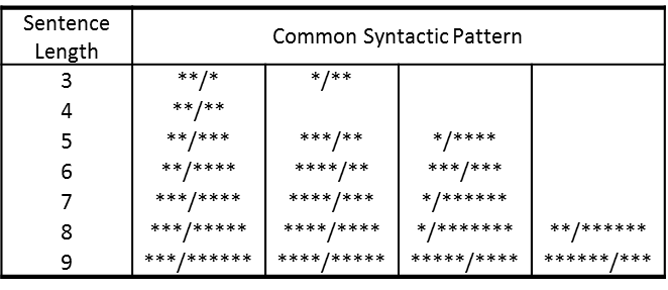
\includegraphics[width=0.9\linewidth]{syntactic.png}
	\caption{Syntactic Patterns for Sentences with Different Length.}
	\label{fig:syntactic}
\end{figure}

Then we defined several properties for characters and words in Song Ci.
%
Tone pattern which is called pingze in Chinese, we use 1 to represent Ping, 2 to represent Ze.
%
There are twenty four rhythm in Chinese, in traditional Chinese poem, usually the last characters of every sentence are required to be the same rhythm.
%
 We get pingze and rhythm information from existing datasets.
%
The correlation between words we use python package word2vec(https://code.google.com/archive/p/word2vec/) to quantify the relationship between words, which will be later used in generating Song Ci that is closely related with keywords.


We also extract format for different Cipai from existing dataset, which contains sentence number, length, tone pattern and the delimiter of each sentence.
%
For example, Huanxisha is a very popular Cipai in Song Ci.
%
The sentence format of Huanxisha is ['0201021', '0102211', '0102211', '0201122', '0102211', '0102211'].
%
In this format, there are 6 sentences, each sentence contains 7 characters.
%
0,1 and 2 represent the requirement of Pingze, 0 means both ping and ze will work in this position.
%
Each sentence will apply the syntactic pattern previous defined.


\begin{figure}[htbp]
	\centering
	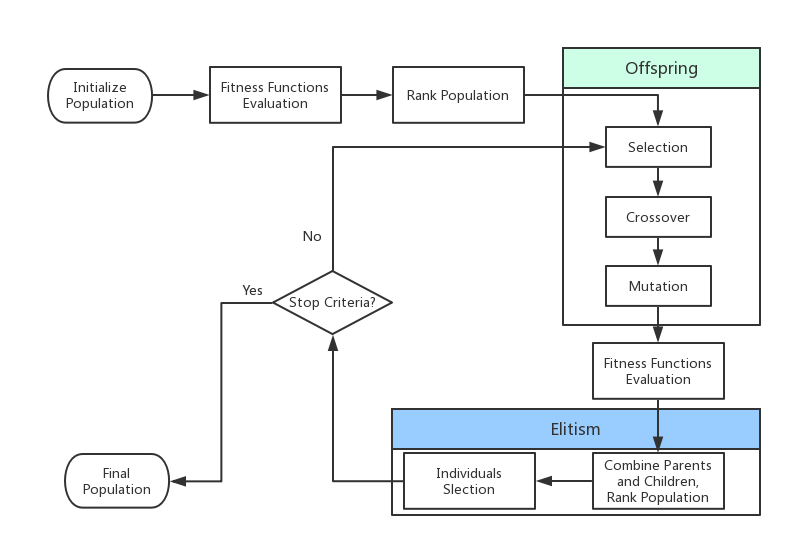
\includegraphics[width=0.9\linewidth]{GA.png}
	\caption{Process of Generating Song Ci by Genetic Algorithm}
	\label{fig:GA}
\end{figure}


Based on the rule of compose Song Ci, we found that Song Ci is a combination of words.
%
Thus, traditional method with pre-defined rules can easily generate Song Ci with correct format.
%
For genetic algorithm, we use a Cipai title and several keywords as input.
%
Based on the sentence format and tone requirement, words that are highly correlated with keywords are selected as candidate words for initial population.
%
Based on randomly chosen rhythm, pre-defined sentence form, syntactic patterns and tone patterns, program randomly put words that satisfied all the requirement to each position and generate the first generation of candidate poems.
%
The initial population is strictly follows the format and rules of Song Ci.


Then all candidate poems go through the fitness evaluation process.
%
Based on score of syntactic and semantic correctness, correlation with keywords, correlation between sentences and tone, rhythm pattern, a fitness value is generated for each candidate poem.
%
Best several individuals are selected as parents to generate offspring with mutation and crossover.
%
Mutation means characters within this poem will change randomly.
%
Crossover represents two poems randomly exchange part of their sentences and form two new poems.
%
All offspring and parents together forms the next generation and need to be evaluate on fitness value.
%
Then this iteration will continue until satisfactory fitness level has been reached or a maximum number of generations has been produced.


In the last, we'll manually choose best poem from the final generation.
%
The whole process is shown in Figure \ref{fig:GA}.
%
Final results are shown in following section.


\subsection{Implementation of a Word Embedding Model }
A word embedding model represent words in a continuous vector space where semantically similar words are mapped to nearby points.
%We implemented this model to find the semantic relations between each Chinese character, so that given a few of keyword characters, such as 'spring' and 'beauty', we can generate poetries with coherent meanings using characters which are close to these keywords in the vector space.
%
%We use a predictive method to implement this  model based on the TensorFlow programming package \cite{tensorflow}.
%
We give a visualized result in Figure \ref{fig:VSM}. 
%
Each of the Chinese characters is embedded into a 2-D space, which are randomly chosen from the most frequent 500 Chinese characters in the Song Ci corpus. The 2-D space corresponds to the first two dimensions in the vector space. We can see that words such as `spring', `sunny', and `breeze' are very close in the 2-D space, which convey similar sentimental feelings to readers.

\begin{figure}[htbp]
	\centering
	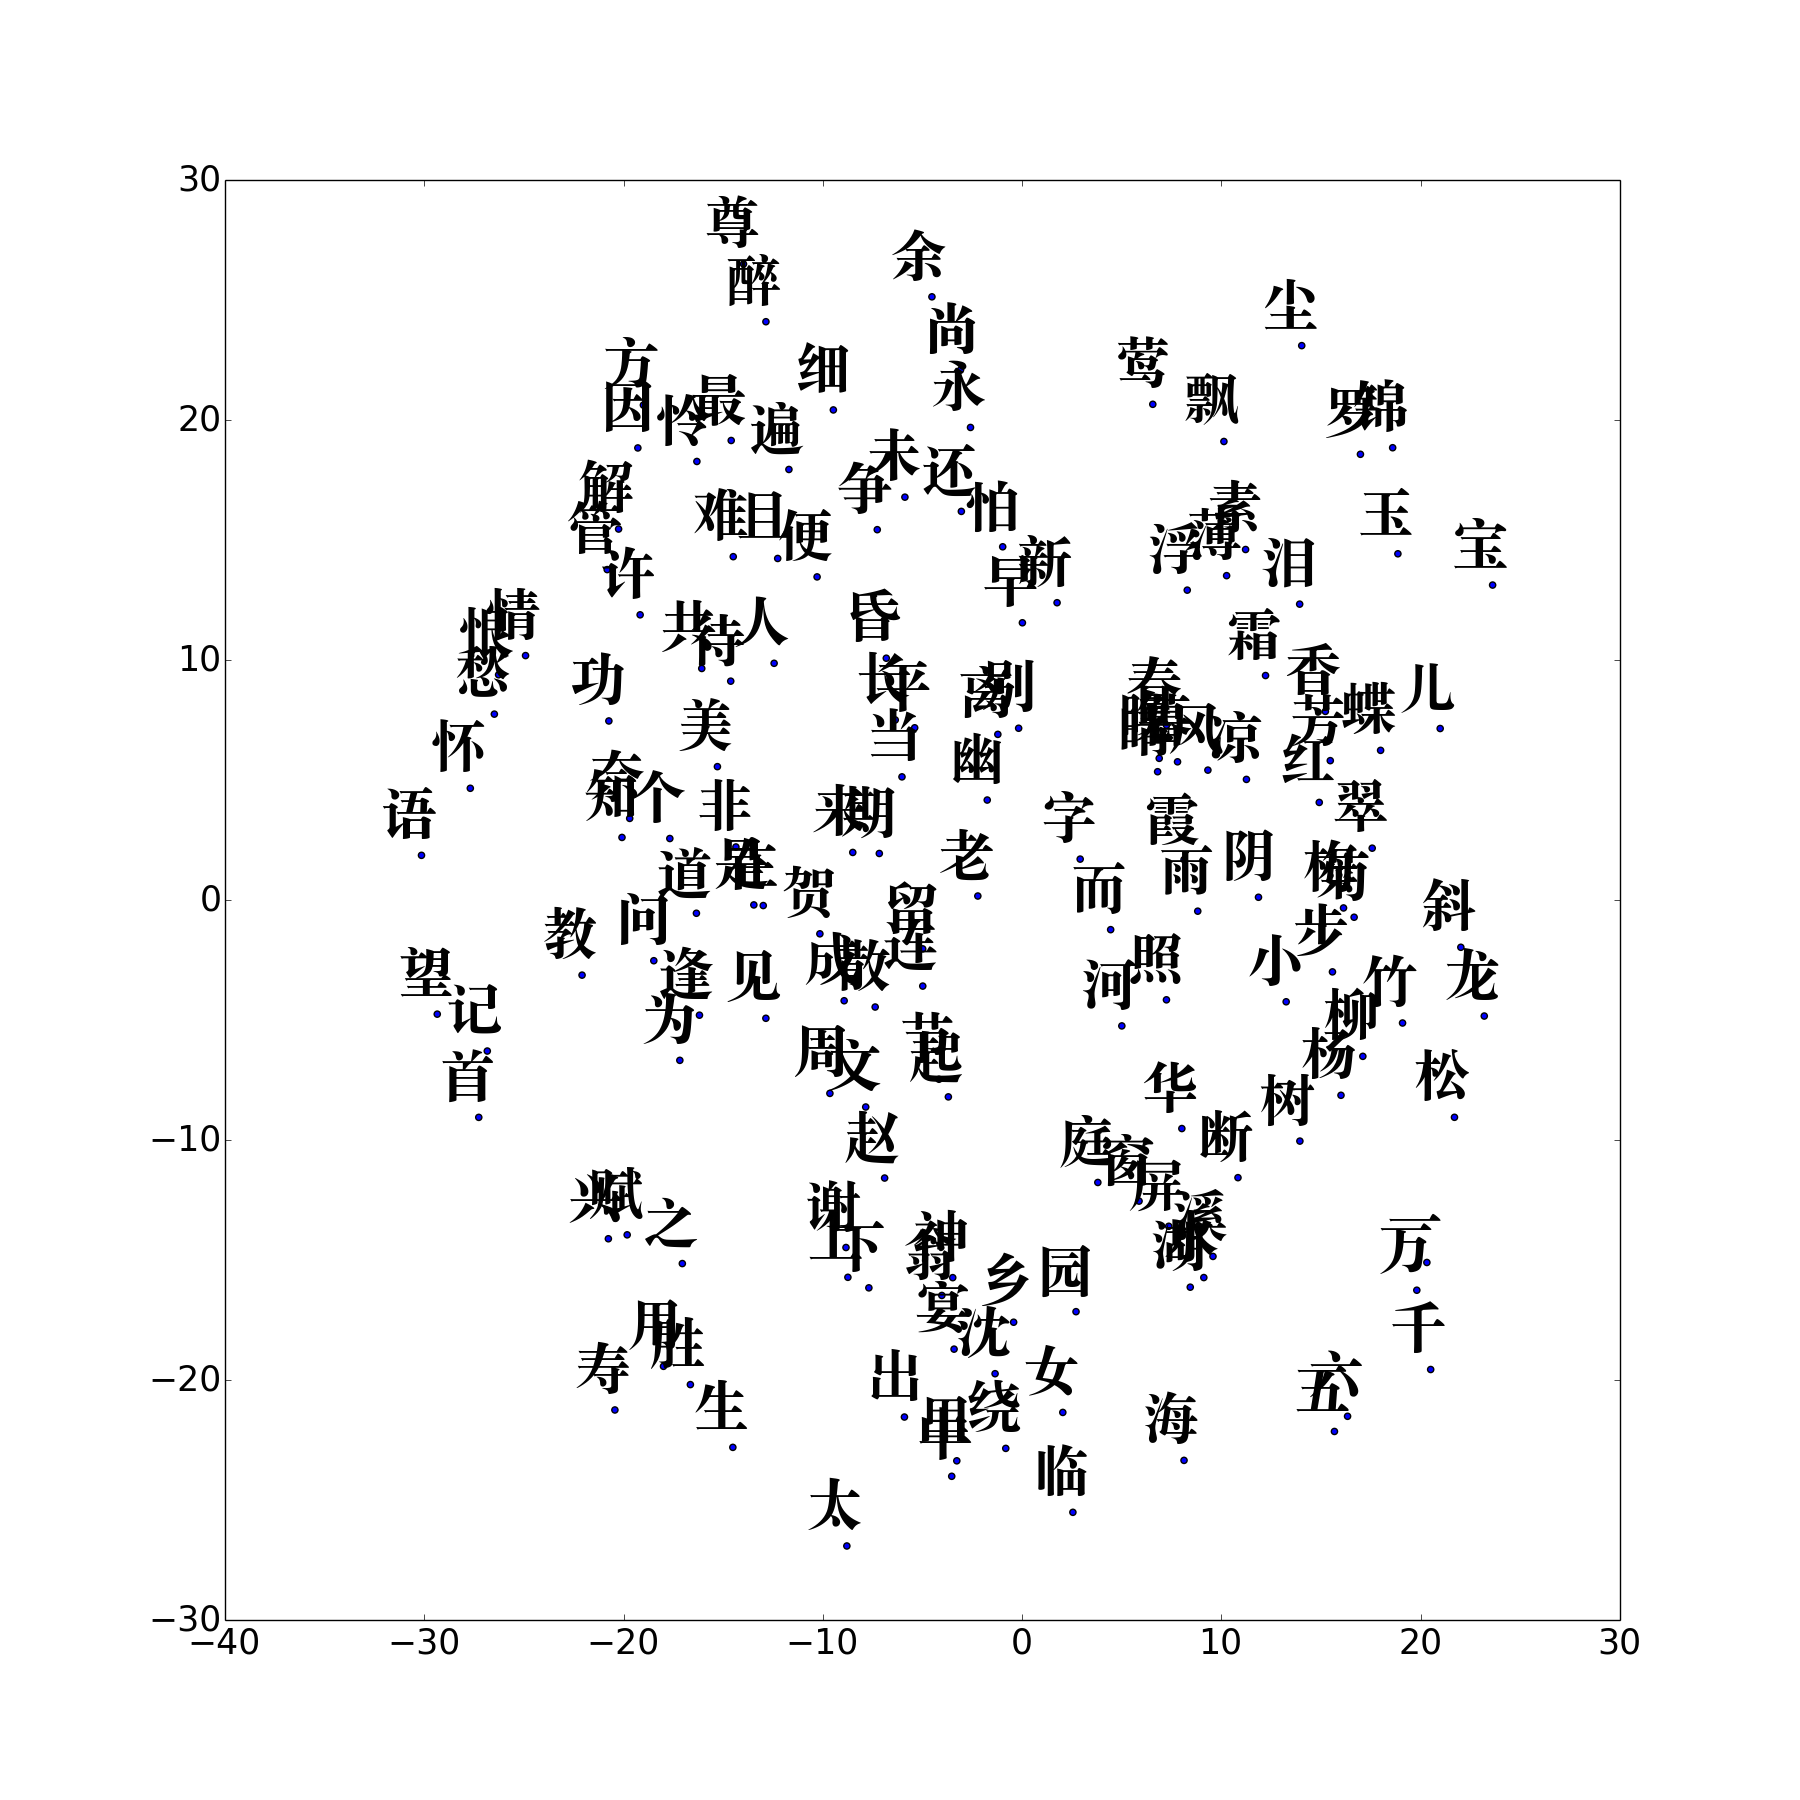
\includegraphics[width=1\linewidth]{tsne.png}
	\caption{Projections of most frequent characters to a 2-D space using the word embedding model}
	\label{fig:VSM}
\end{figure}


\subsection{Implementation of an RNN Model} 
%
We used deep learning Python modules called \emph{TensorFlow} \cite{tensorflow} to implement our RNN model. The core parameters are given in Table \ref{fig:rnn_workflow}.
%
The core of the model consists of an LSTM cell that processes one word at a time and computes probabilities of the possible values for the next word in the sentence. 
%
The general workflow of our model is shown in Figure \ref{fig:rnn_workflow}.
%
The memory state of the network is initialized with a vector of zeros and gets updated after reading each word. 



\begin{figure}[htbp]
	\centering
	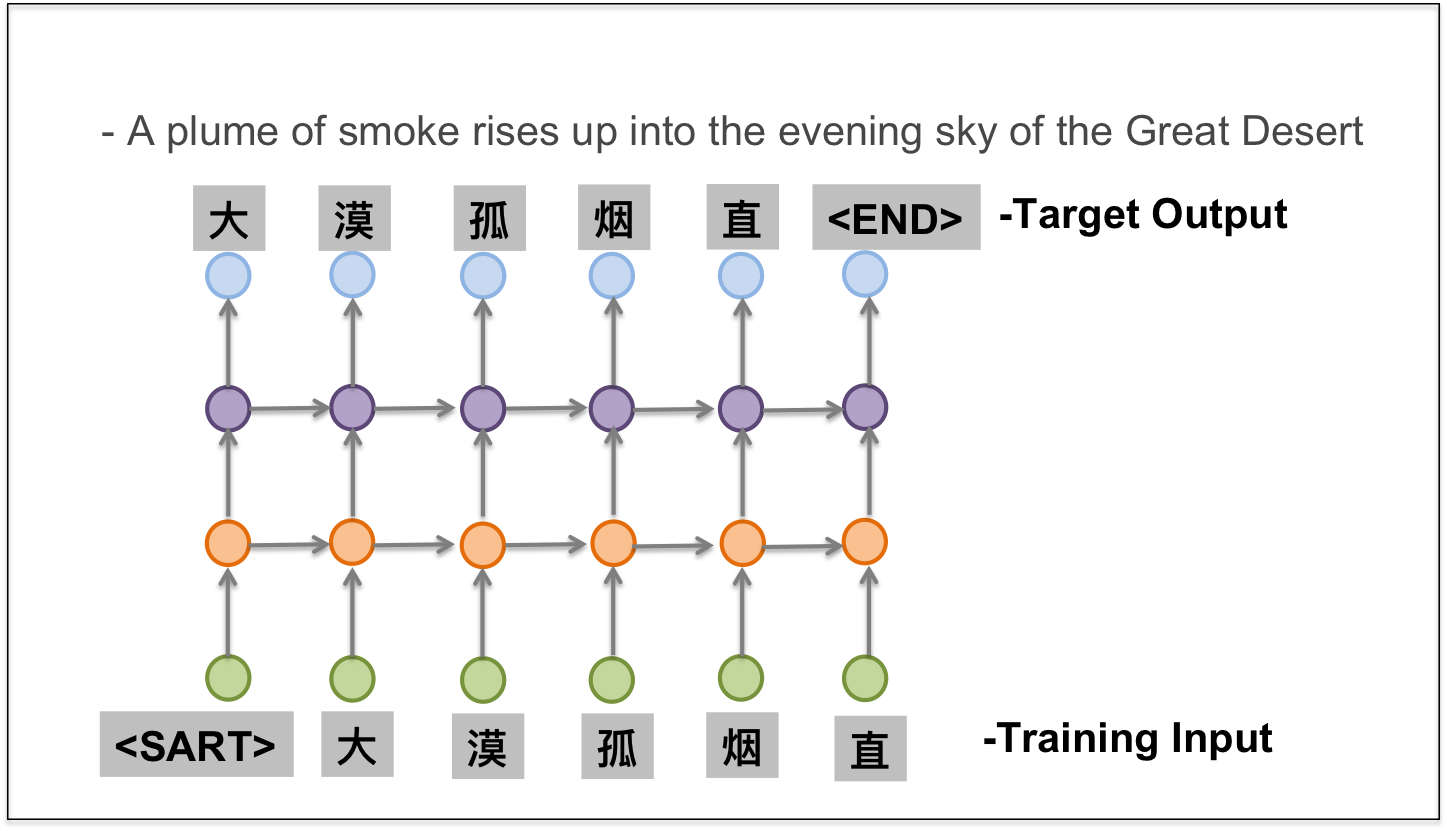
\includegraphics[width=0.9\linewidth]{RNN_model}
	\caption{Workflow of the RNN model}
	\label{fig:rnn_workflow}
\end{figure}

\begin{table}[htpb]
\centering
\caption{RNN model parameters}
\label{table:rnn}
\begin{tabular}{|l|l|}
\hline
\textbf{Parameter}      & \textbf{Value} \\ \hline
\textbf{batch\_size}    & 64             \\ \hline
\textbf{embedding size} & 64             \\ \hline
\textbf{hidden layer}   & 48             \\ \hline
\textbf{dropout rate}   & 0.8            \\ \hline
\textbf{learning rate}  & 0.0001         \\ \hline
\textbf{epoch time}     & 50             \\ \hline
\end{tabular}
\end{table}

\begin{itemize}
\item \textbf{Batch Input.} We want to train the RNN model in an iterative fashion, so the first step is to seperate the training set into different batches with the same size. The larger the batch, the less epoch time the model needs to finish training. In our model, we tune the batch size to be 64, so each time a set of 64 Song Ci will be used as the input to our model, and the value of the model state is updated after processing each batch of texts.

\item \textbf{Truncated Backpropagation.} In order to make the learning process tractable, it is important to create an unrolled version of the network which contains a fixed number of LSTM inputs and outputs, known as the number of steps. The model is then trained on this finite approximation of the RNN. 
%
In our model, we tune the number of steps to be the ideal character length in the Song Ci with a specified Ci Pai. For example, in order to train a Song Ci with Ci Pai ''Sandy Creek Washers", we set this number to be 48, because the input Song Ci is all of length 48 at a time.
%
Then we can perform a backward pass after each such input block.

\item \textbf{Optimizing Loss Function.} We aim to minimize the average negative log probability of the target words: 
\begin{align*}
\text{loss} = -\frac{1}{N} \sum_{i=1}^{N} \ln p_{target_i}
\end{align*}
We implement by using \emph{TensorFlow} 's \emph{seq2seq} library. It will generate the weighted cross-entropy loss for a sequence of logits, based on three inputs: the logits, the targets, and the weights. 

 
\item \textbf{Stacking Multiple LSTMs.} We  use multiple layers of LSTMs to process the data so that the output of the current layer will become the input of its succesor.
%
In our model,  we use the libray called \emph{MultiRNNCell} to implement three LSTM networks to strike a balance between the training time and the quality of the model output.
\end{itemize}

\subsection{Implementation of SeqGAN Model.} 

The SeqGAN model is implemented using TensorFlow \cite{tensorflow}. We first read all the data from text files, then convert all the Chinese character to integer vectors. Since Ci has different length, we also use the special placeholder to fill the space after the end of the text. The sequence length is adjusted based on task. For general Ci generation, we use 128 as sequence length. For Huanxisha generation, we use 48 as sequence length. We use an adaptive learning optimization algorithm called Adam \cite{kingma2014adam} to optimize our CNNs with initial learning rate $ =  0.01 $.

For the generator, we use LSTM cell \cite{hochreiter1997lstm} as the unit of hidden layers of recurrence neural networks. Right now, our implementation has 64 units in the hidden layers of RNNs.

The discriminator is a convolutional neural network for 2 classes classification. The input matrix is from the embedding of discrete tokens. Convolutional kernel applied to the input matrix to extract features. In our implementation, all convolution operation use $ [1, 1, 1, 1]  $ as its strides and valid padding. In the real implementation, a series of the diffrent number of the convolutional kernel with different window size is applied to extract different features. The model also adopt highway structure \cite{srivastava2015highway} and dropout (dropout rate $ = 0.25 $)\cite{hinton2012dropout} to further improve the performance. The loss function of CNNs is cross entropy loss function with l2 norm regularization term. In the experiment, the coefficient of l2 norm $ \lambda =  0.2 $. We use an adaptive learning optimization algorithm called Adam \cite{kingma2014adam} to optimize our CNNs with initial learning rate $ =  1e^{-4} $. We still use Adam optimizer with $ 1e^{-4} $ as its learning rate.

To train the SeqGAN model, we use the computational node provided by High-Performance Computing Center from Michigan State University. Most training job running use a single Nvidia Tesla K80 GPU in the  intel16-k80 clusters. For Huanxisha generation, a 12-hour job generates 79000 poems.
 

 

\subsection {Results Comparision}
We present  the Song Ci generated by our three models respectively, as shown in Figure \ref{fig:poem_template}, Figure \ref{fig:poem_template2}, and Figure \ref{fig:poem_template3}. We evaluate the quality of our results based on human evaluation by 3 graduate students.

For both results generated by GA and RNN model, they maintain good property on the structure as well as rhythmic constraints. %
They also convey consistent meanings with poetic semantics. For GAN model, the good performance relies on carefully designed rules and constraints and a evaluation function. 
%
For RNN model, the good performance relies on a large set of training data, so that the structure or rhyme rules can be captured automatically.

For results generated by GAN model, it maintains the correct structure and gramma rules, but it does not capture the rhythmic patterns nor the semantic consistency.

 \begin{figure}[ht]
\begin{minipage}[t]{1.1\linewidth}
\centering 
\subfigure[A Song Ci generated using Genetic Algorithm]{
   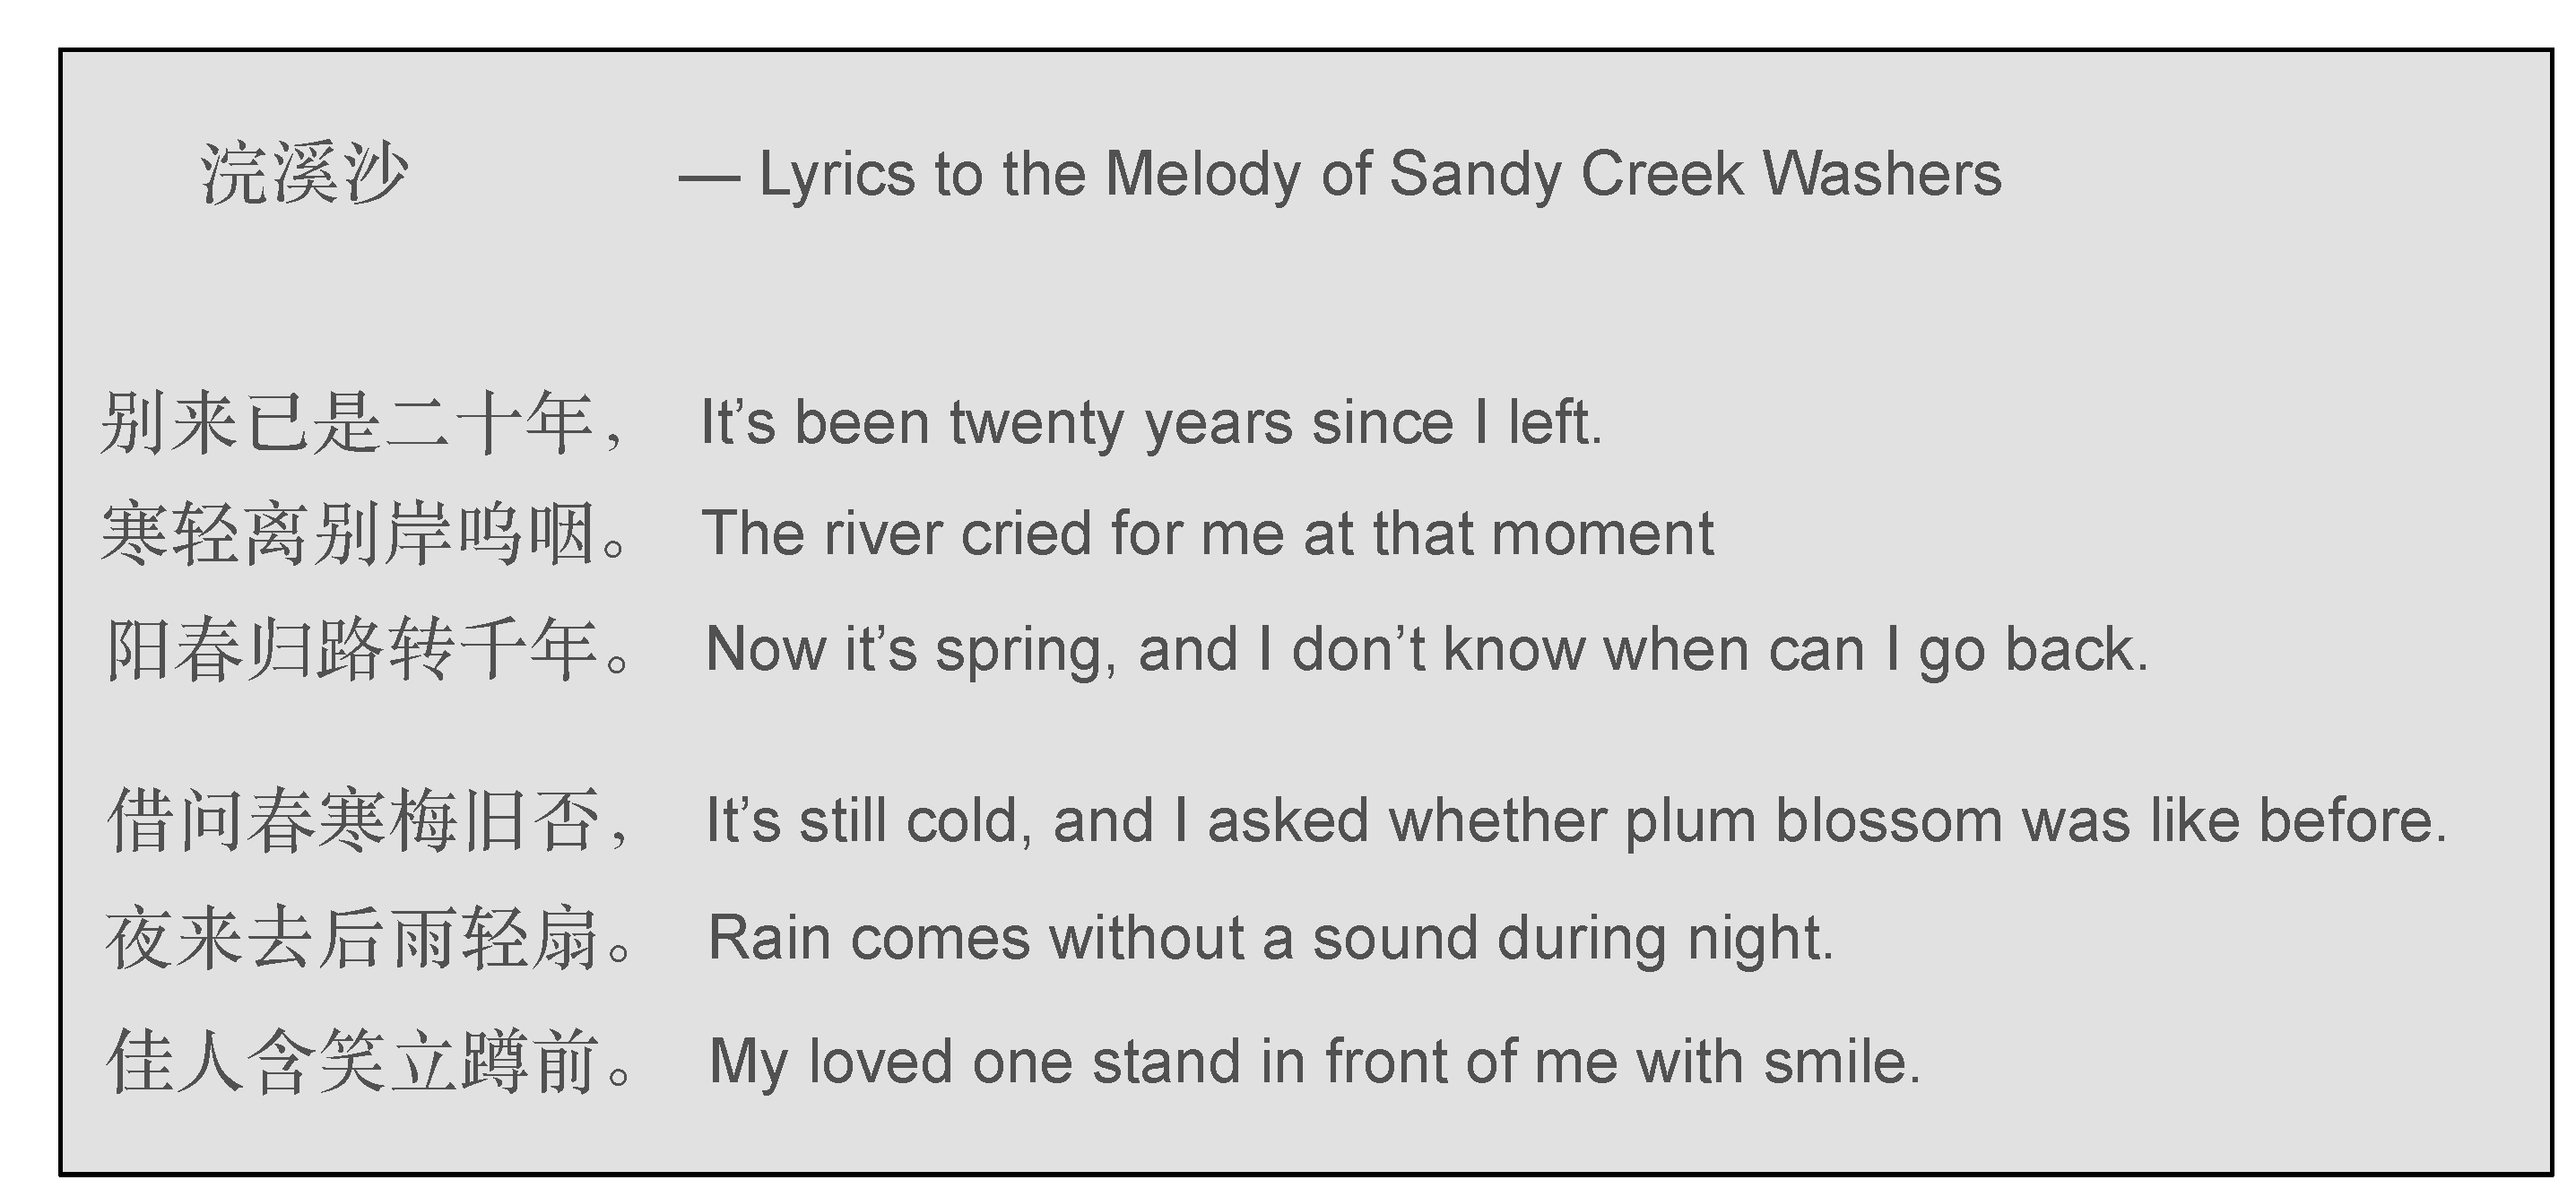
\includegraphics[width=1\linewidth] {poem_template2}
   \label{fig:poem_template2}
 }
 
 \subfigure[A Song Ci generated using LSTM]{
   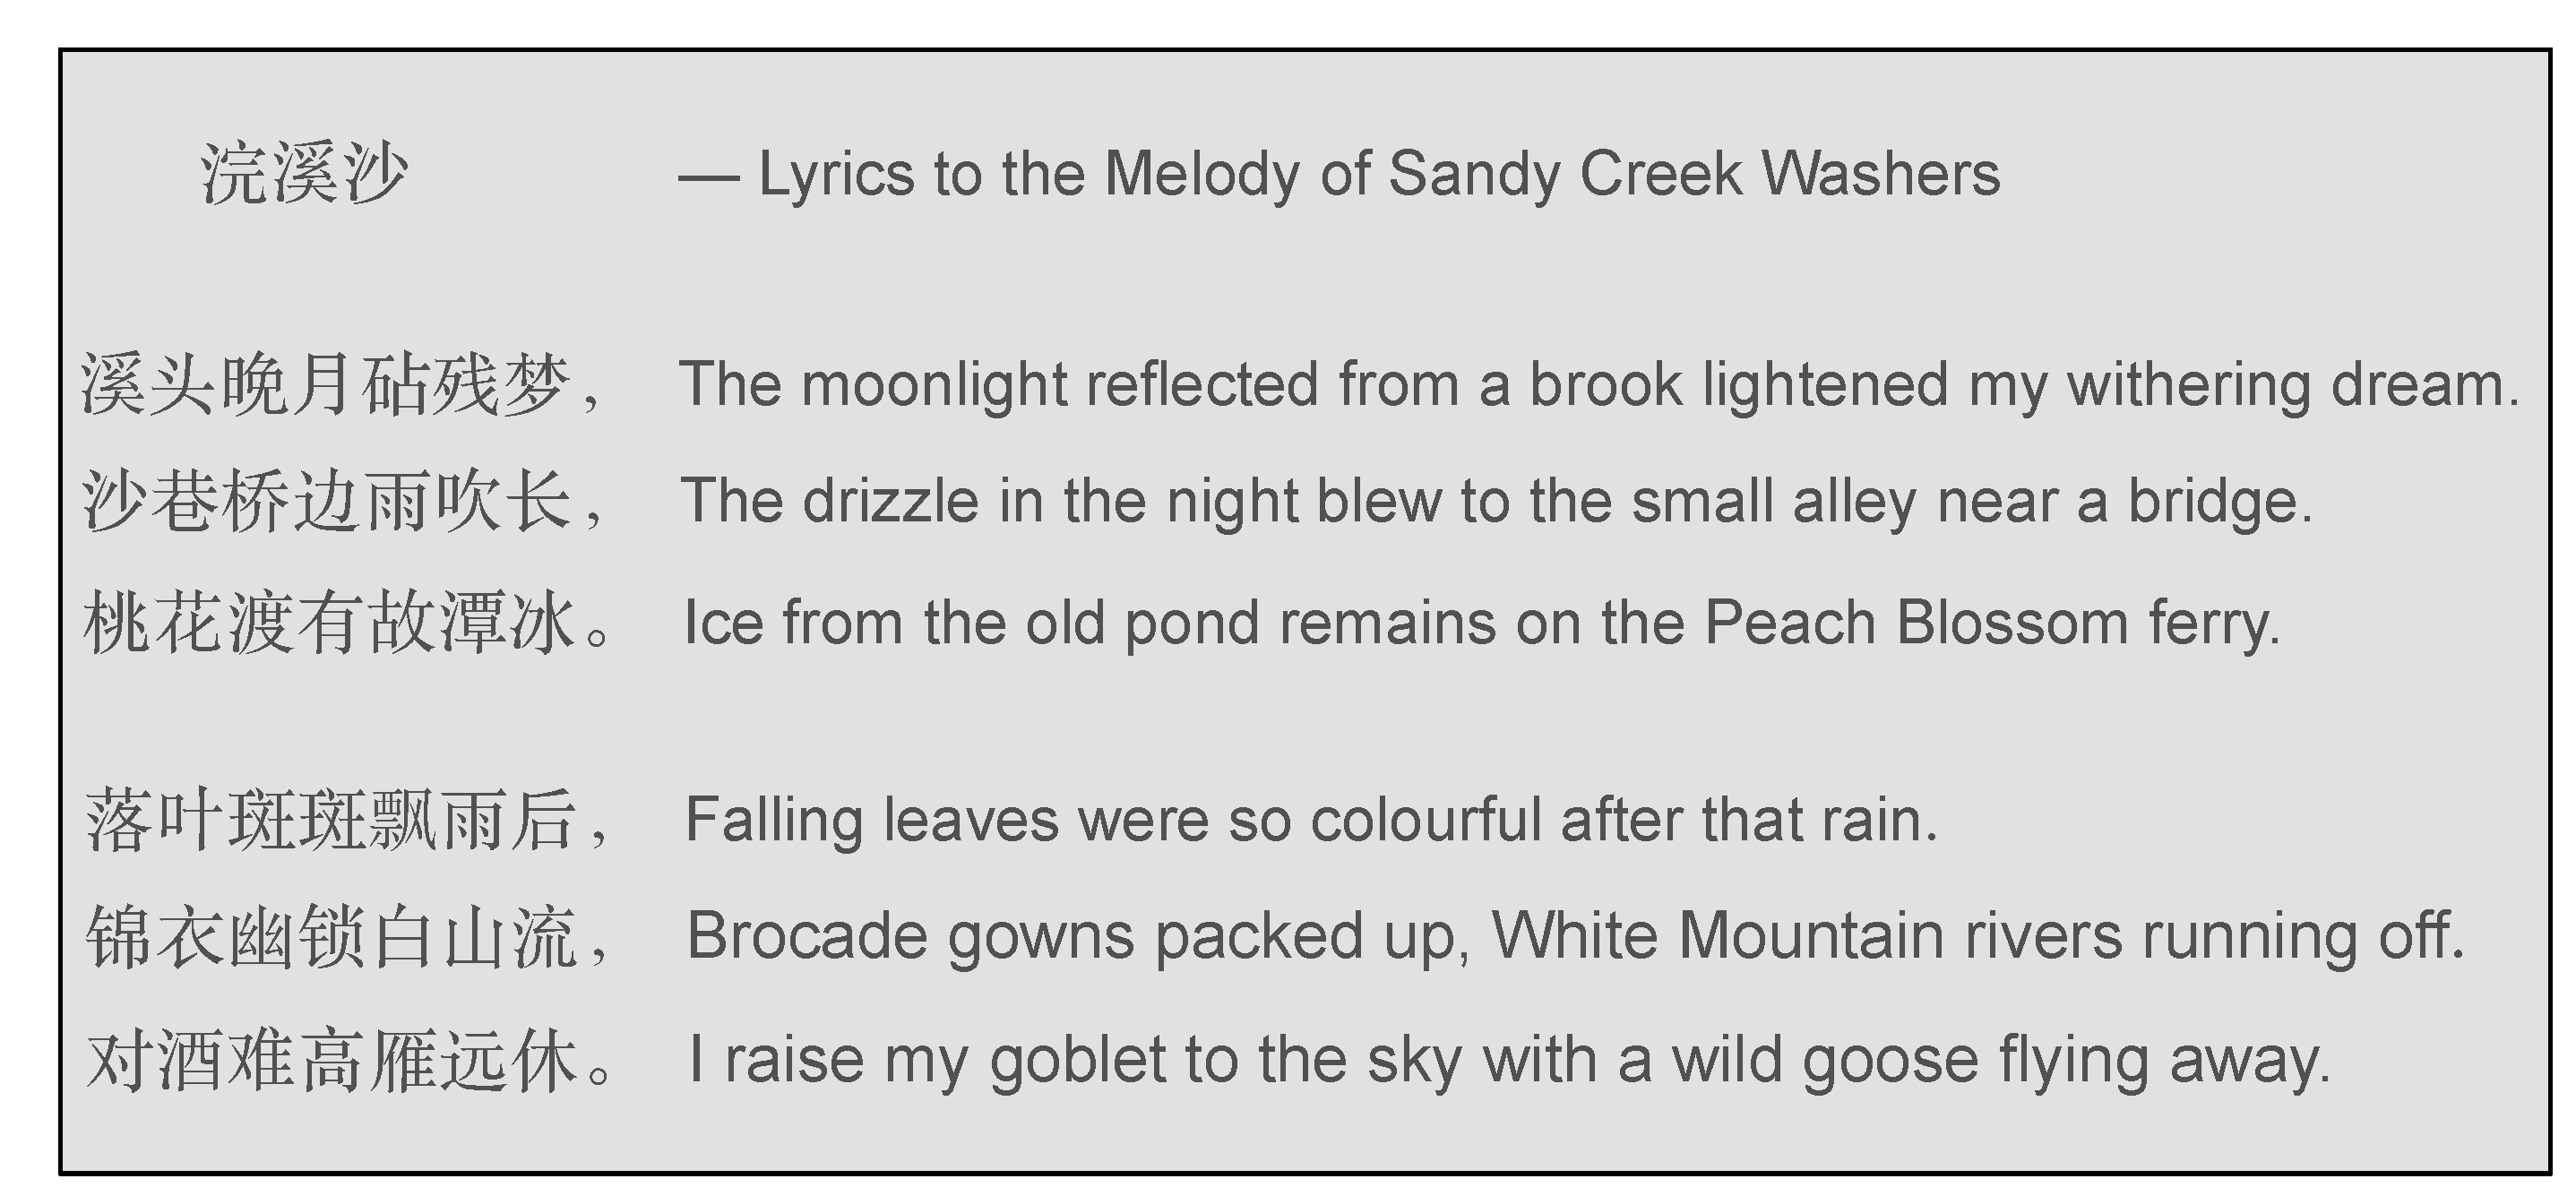
\includegraphics[width=1\linewidth] {poem_template}
   \label{fig:poem_template}
 } 
 
 \subfigure[A Song Ci generated using GAN]{
   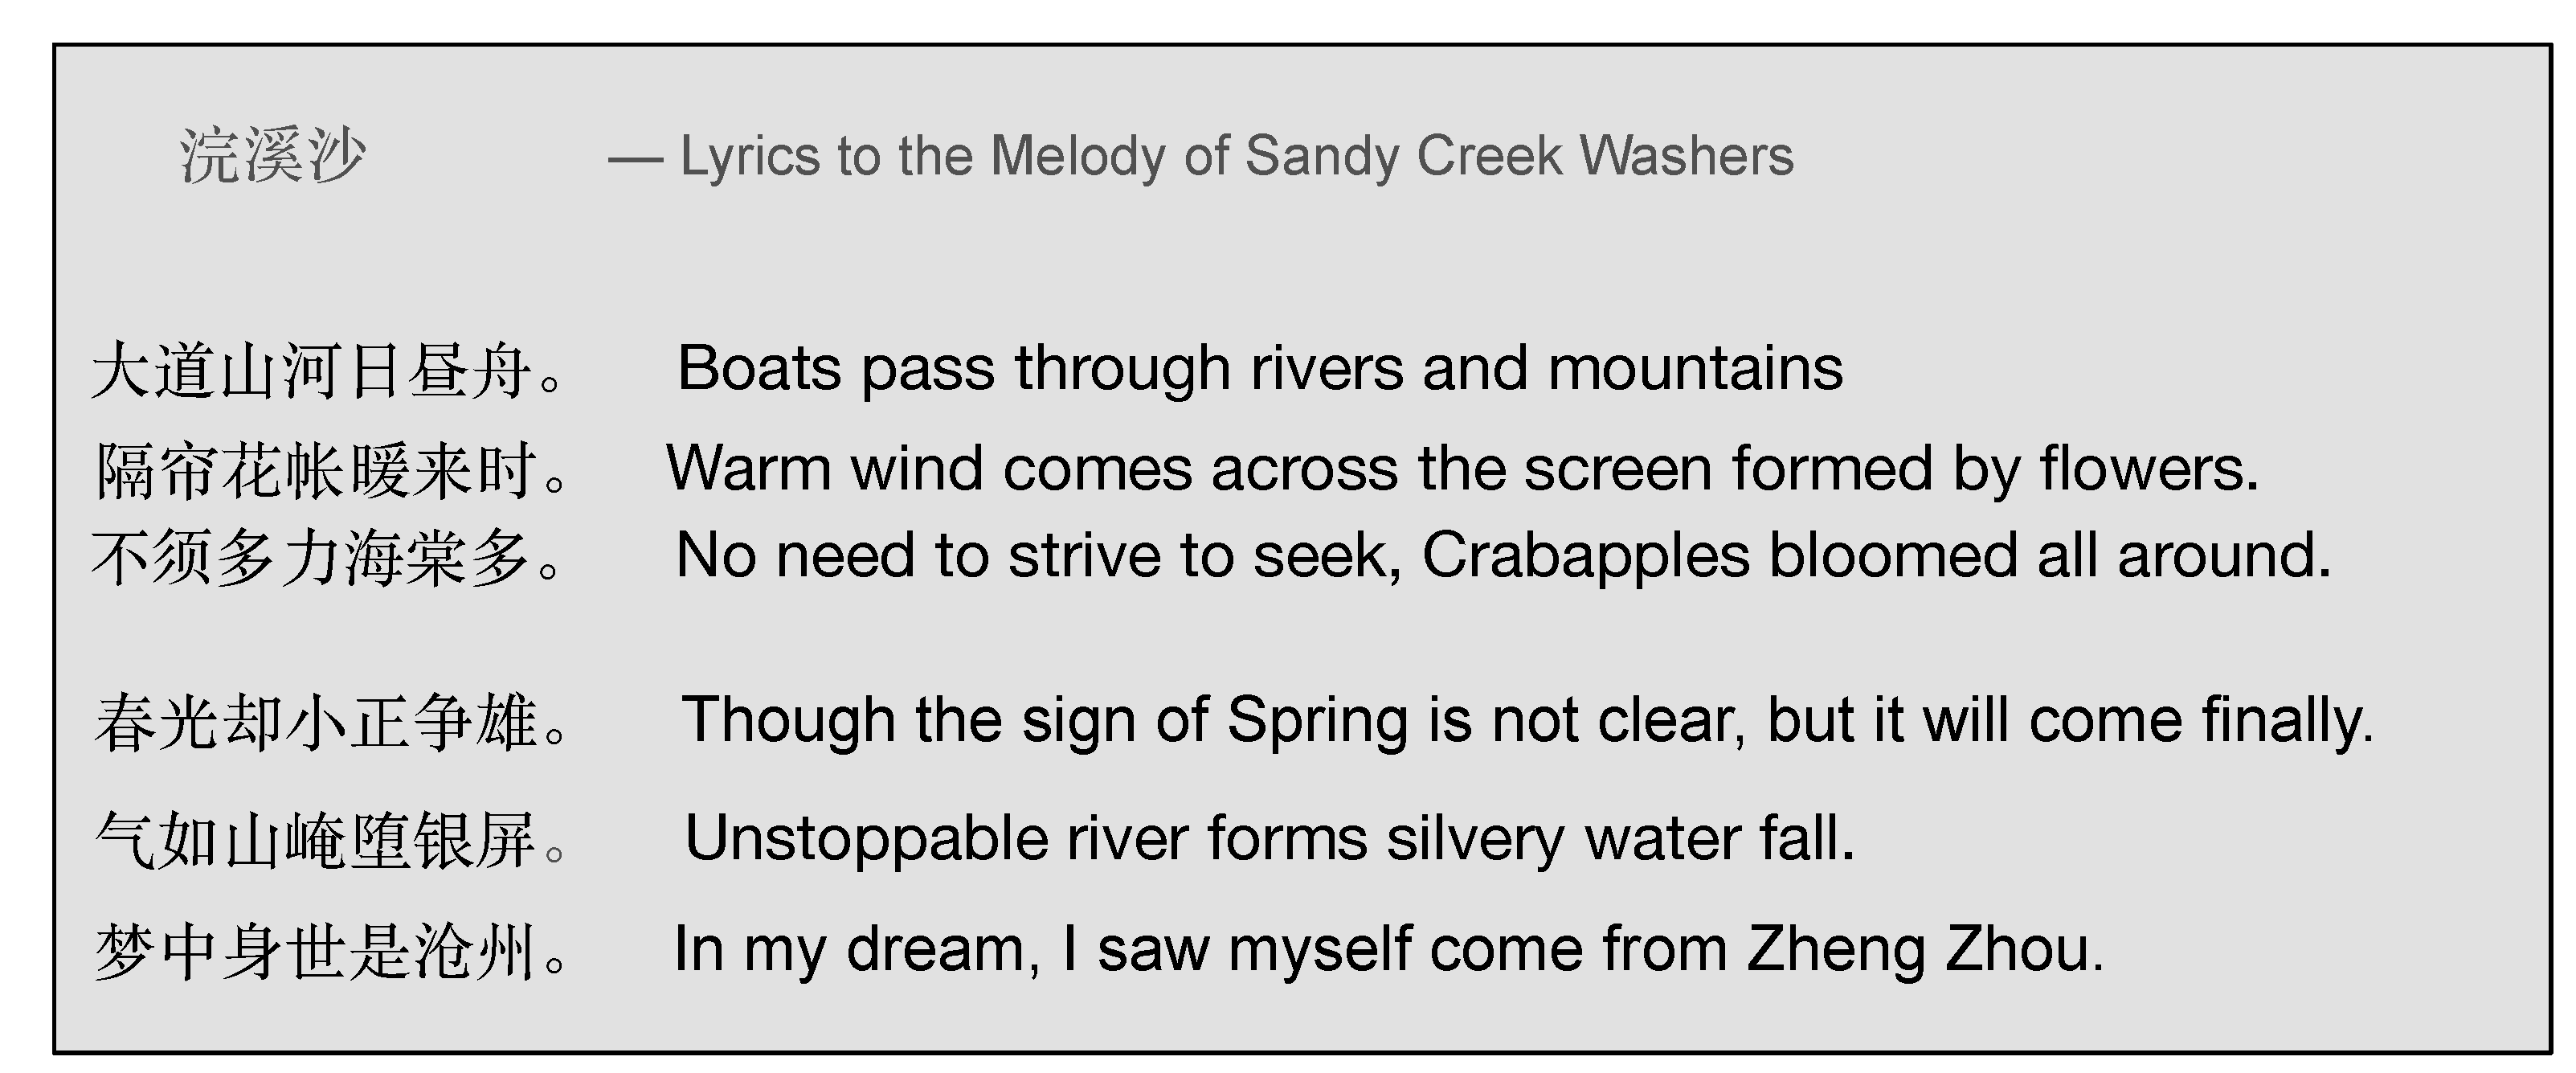
\includegraphics[width=1\linewidth] {poem_template3}
   \label{fig:poem_template3}
 } 
\caption{\textbf{Song Ci generated Using Three Different Approaches}}
\label{fig:songci}
\end{minipage}
\end{figure}


 